%%%%%%%%%%%%%%%%%%%%%%%%%%%%%%%%%%%%%%%%%%%%%%%%%%%%%%%%%%%%%%%
%%%  pta notes
%%%%%%%%%%%%%%%%%%%%%%%%%%%%%%%%%%%%%%%%%%%%%%%%%%%%%%%%%%%%%%%

\documentclass[onecolumn,fleqn,longbibliography]{revtex4}

% fonts
\usepackage{latexsym}
\usepackage{amsmath} 
\usepackage{amssymb} 
\usepackage{bm}
\usepackage{wasysym}

\usepackage{graphicx}


% extra by jarondl

\usepackage{array}
\usepackage{float}%unfloats
%\usepackage{multicol}
\usepackage[caption=false]{subfig} %subcaption is not compat with revtex
\usepackage[pdftitle={PTA},bookmarks]{hyperref}

%%%%%%%%%%%%%%%%%%%%%%%%%%%%%%%%%%%%%%%%%%%%%%%%%%%%%%%%%%%%%%%%

% NEW 
\newcommand{\abs}[1]{\left|#1\right|}
\newcommand{\varphiJ}{\bm{\varphi}}
\newcommand{\thetaJ}{\bm{\theta}}
%\renewcommand{\includegraphics}[2][0]{FIGURE}
\newcommand{\rmrk}[1]{\textcolor{red}{#1}}
\newcommand{\Eq}[1]{\textcolor{blue}{Eq.\!\!~(\ref{#1})}} 
\newcommand{\Fig}[1]{\textcolor{blue}{Fig.}\!\!~\ref{#1}}

% math symbols I
\newcommand{\sinc}{\mbox{sinc}}
\newcommand{\const}{\mbox{const}}
\newcommand{\trc}{\mbox{trace}}
\newcommand{\intt}{\int\!\!\!\!\int }
\newcommand{\ointt}{\int\!\!\!\!\int\!\!\!\!\!\circ\ }
\newcommand{\ar}{\mathsf r}
\newcommand{\im}{\mbox{Im}}
\newcommand{\re}{\mbox{Re}}

% math symbols II
\newcommand{\eexp}{\mbox{e}^}
\newcommand{\bra}{\left\langle}
\newcommand{\ket}{\right\rangle}

% Mass symbol
\newcommand{\mass}{\mathsf{m}} 
\newcommand{\rdisc}{\epsilon} 

% more math commands
\newcommand{\tbox}[1]{\mbox{\tiny #1}}
\newcommand{\bmsf}[1]{\bm{\mathsf{#1}}} 
\newcommand{\amatrix}[1]{\begin{matrix} #1 \end{matrix}} 
\newcommand{\pd}[2]{\frac{\partial #1}{\partial #2}}

% equations
\newcommand{\mylabel}[1]{\label{#1}} 
\newcommand{\beq}{\begin{eqnarray}}
\newcommand{\eeq}{\end{eqnarray}} 
\newcommand{\be}[1]{\begin{eqnarray}\ifthenelse{#1=-1}{\nonumber}{\ifthenelse{#1=0}{}{\mylabel{e#1}}}}
\newcommand{\ee}{\end{eqnarray}} 

% arrangement
\newcommand{\hide}[1]{}
\newcommand{\drawline}{\begin{picture}(500,1)\line(1,0){500}\end{picture}}
\newcommand{\bitem}{$\bullet$ \ \ \ }
\newcommand{\Cn}[1]{\begin{center} #1 \end{center}}
\newcommand{\mpg}[2][1.0\hsize]{\begin{minipage}[b]{#1}{#2}\end{minipage}}
\newcommand{\mpgt}[2][1.0\hsize]{\begin{minipage}[t]{#1}{#2}\end{minipage}}

%%%%%%%%%%%%%%%%%%%%%%%%%%%%%%%%%%%%%%%%%%%%%%%%%%%%%%%%%%%%%%%%%%%%%%%%%%%
% Sections
\newcommand{\sect}[1]
{
\addtocounter{section}{1} 
\setcounter{subsection}{0}
\ \\ 
\pdfbookmark[2]{\thesection. \ #1}{sect.\thesection}
{\Large\bf $=\!=\!=\!=\!=\!=\;$ [\thesection] \ #1}  
\nopagebreak
}

% subections
\newcommand{\subsect}[1]
{
\addtocounter{subsection}{1} 
\ \\ 
\pdfbookmark[2]{\ \ \ \ \thesection.\thesubsection. \ #1}{subsect.\thesection.\thesubsection}
{\bf $=\!=\!=\!=\!=\!=\;$ [\thesection.\thesubsection] \ #1}  
\nopagebreak
}
%%%%%%%%%%%%%%%%%%%%%%%%%%%%%%%%%%%%%%%%%%%%%%%%%%%%%%%%%%%%%%%%%%%%%%%%
%%%%%%%%%%%%%%%%%%%%%%%%%%%%%%%%%%%%%%%%%%%%%%%%%%%%%%%%%%%%%

\graphicspath{{figures/}}
\begin{document}

\title{PTA}

\author{YdL}

\maketitle

%%%%%%%%%%%%%%%%%%%%%%%%%%%%%%%%%%%%%%%%%%%%%%%%%%%%%%%%%%%%%%%%%%%%%%%%
%%%%%%%%%%%%%%%%%%%%%%%%%%%%%%%%%%%%%%%%%%%%%%%%%%%%%%%%%%%%%%%%%%%%%%%%


%%%%%%%%%%%%%%%%%%%%%%%%%%%%%%%%%%%%%%%%%%%%%%%%%%%%%%%%%%%
\sect{Model}

We wish to study a banded model similar to the one presented in \cite{bodyfelt_scaling_2013},
starting with an ordered (and periodic) matrix:
%
\begin{align}\label{eq:ordered}
w_{nm} &= \begin{cases}
  w_0 &\qquad \textrm{ if  } \quad 0<|n-m|\le 1 \\
  0 &\qquad \textrm{ otherwise}
\end{cases}
\end{align}
%
According to Bloch's theorem, the eigenvectors of translational invariant
matrices are plane waves, and their eigenvalues can be easily deduced:
\begin{align}
k\ \  &=\ \  \frac{\pi m}{N} \ \ \ \ \ m=1..N \\
\vec{V}_k\ \  &=\ \  \cos(k\cdot x)\\
\lambda_k\ \  &=\ \  \sum_{n=1..b} 2\cos(n\cdot k) \\
&= \ \ -1 + \frac{\sin((b+\dfrac{1}{2})k)}{\sin(\dfrac{1}{2}k)}
\end{align}  
Where in the last step we have used one of Lagrange's trigonometric identities. 
The lower bound of $lambda_k$ is $-2b$. 
$\lambda_k$ for several values of $b$ is plotted in \autoref{fig:theor_banded_ev}.

%%%%%%%%----------%%%%%%%%
%%%%%%%%  figure  %%%%%%%%
%%%%%%%%----------%%%%%%%%
\begin{figure}[H]
    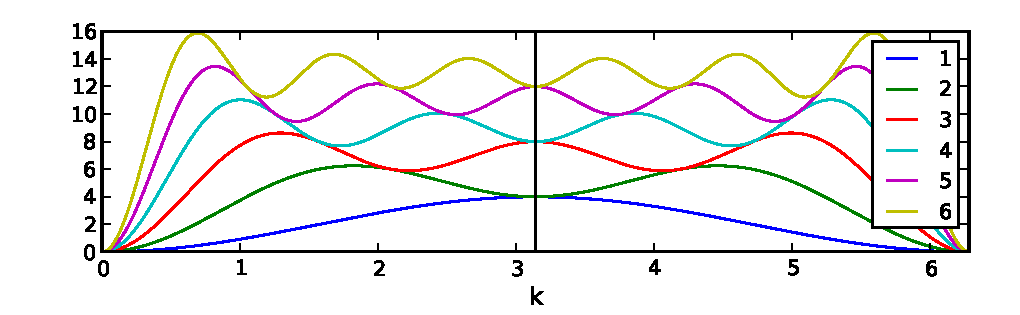
\includegraphics{pta_theor_banded_ev}
    \caption{$\lambda(k)$ for banded ordered matrices. Both plots
    represent the same curves, but in the left one there is a $+2b$ shift, both for clarity 
    and for later usage in conservative matrices. Since our 
    models are periodic, only the left half ($0,\pi$) of each plot is relevant. Since 
    the tangent is $DOS^{-1}$, the points with tangent zero are $DOS$ divergences.
    }
    \label{fig:theor_banded_ev}
\end{figure}



A cosine plane wave will have $PN= \frac{2}{3}N$. We can also compute the mode velocity:
\begin{align}
v \ \ &=\ \ \frac{d\lambda_k}{dk} \ \ =\ \ -\sum_{n=1..b} 2\cdot n\cdot \sin(n\cdot k)
\end{align}
Note that this expression is {\bf not single valued}. Meaning that each $\lambda$ 
has more than one associated velocity. 


The $DOS$ is defined by $\frac{dk}{d\lambda_k}$, which is the inverse of the 
velocity. Since density is additive, for each $\lambda$ we add the densities
of all relevant $k$ modes. For the moment we use a numerical solution to
find those $k$s. In \autoref{fig:dos} we plot the velocities and inverse 
$DOS$ as a function of $lambda$.
%%%%%%%%----------%%%%%%%%
%%%%%%%%  figure  %%%%%%%%
%%%%%%%%----------%%%%%%%%
\begin{figure}[H]
    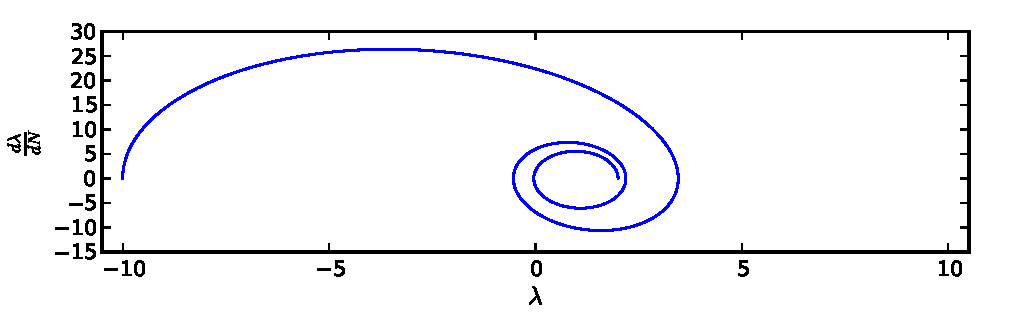
\includegraphics{pta_theor_banded_dos}
    \caption{The velocity and inverse $DOS$ for each eigenvalue $\lambda$, for $b=5$. 
             The inverse $DOS$ will always be less then the velocity. 
             We see large $DOS$ (small inverse) at energies where a single
             mode $DOS$ is diverging, and where we have more than one $k$.}
    \label{fig:dos}
\end{figure}


 
%%%%%%%%%%%%%%%%%%%%%%%%%%%%%%%%%%%%%%%%%%%%%%%%%%%%%
\sect{Adding disorder - finite localization}

The ordered lattice had no localization - all the $PN$ where equal to $\frac{2}{3}N$.
We introduce uniformly distributed diagonal disorder:
\begin{align}
\gamma_n  \ = \  w_{nn} \ \in \ \left[-\frac{s}{2},+\frac{s}{2} \right]
\end{align}

This disorder, as small as it may be, will cause finite Anderson localization.
According to FGR, the transition rate (or the inverse of mean-free-time) is
\begin{align}
\frac{1}{t_\ell} = \varrho \langle w_{nm}^2\rangle
\end{align}
Where $\varrho$ is the Density-Of-States, and $w_{nm}$ is a rate between
neighboring sites.
To get the mean-free-path, we need to translate this to units of distance:
\begin{align}
\ell = v_\lambda t_\ell = \frac{v_\lambda}{\varrho \langle w_{nm}^2\rangle}
\end{align}
As mentioned before, the problem is that $v_\lambda$ is not single valued,
so we do not know yet what should be put there. If we put the inverse of 
the DOS, we get the expression:
\begin{align}
\ell = \frac{\varrho^{-2}}{ \langle w_{nm}^2\rangle}
\end{align}
We plot this result as a solid line in the next figures, with $<w^2> = s^2/3$.
On the eigenvalue axis, it does tell us about eigenvalues with low $PN$,
and the span (or band) where eigenvlaues exist. This does not scale with $N$, although 
the numerics seem to do so \autoref{fig:anderson_byN}

%%%%%%%%----------%%%%%%%%
%%%%%%%%  figure  %%%%%%%%
%%%%%%%%----------%%%%%%%%
\begin{figure}[H]
    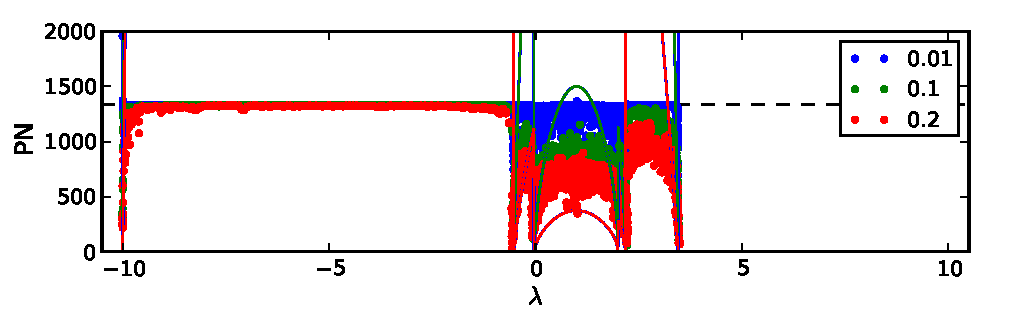
\includegraphics{pta_anderson_ddonly_b5}\\
    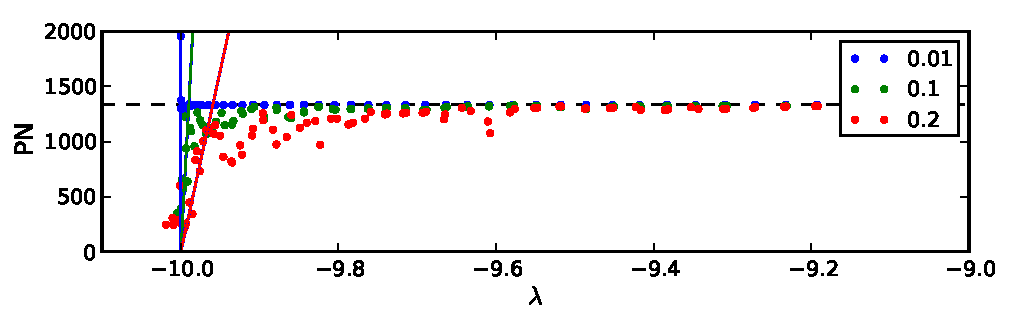
\includegraphics{pta_anderson_ddonly_b5_zoom}
    \caption{$PN$ vs eigenvalue $\lambda$, for $b=5$, $N=2000$. We see that
    no $PN$ is higher than the plane waves' $PN =2/3 N$. We can also explain
    points with low $PN$ by the corresponding $DOS$, and the band of eigenvalues. 
    Compare this to figure 2 of \cite{bodyfelt_scaling_2013}. The 
    differences are that there the basic matrix (before disorder) had a 'conserving' diagonal of $-2b$,
    which corresponds to a horizontal shift, the $x$-axis there is $\sqrt{\lambda}$,
    the disorder is over the main $2b+1$ diagonal instead of only the main diagonal, 
    and the disorder is larger, $s=0.5$.}
    \label{fig:ddonly_b5}
\end{figure}


%%%%%%%%----------%%%%%%%%
%%%%%%%%  figure  %%%%%%%%
%%%%%%%%----------%%%%%%%%
\begin{figure}[H]
    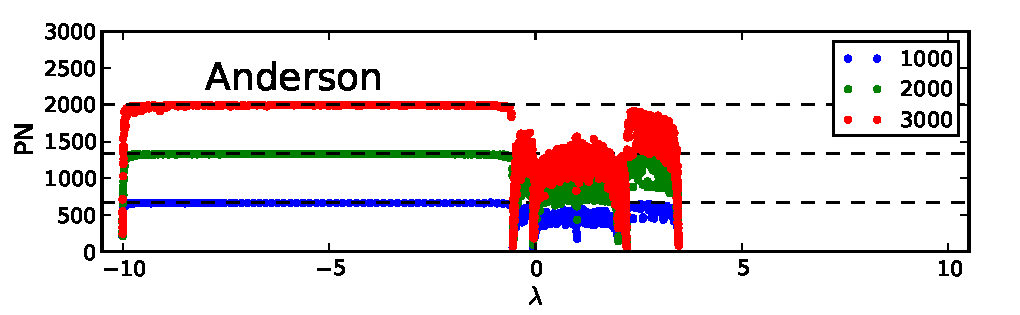
\includegraphics{pta_anderson_byN}
    \caption{$PN$ vs eigenvalue $\lambda$, for $b=5$, $s=0.1$ ,$N={{1000,2000,3000}}$. 
    Here we see the scaling in $N$ of the $PN$ values. The $PN$ of the 
    larger left portion scales as expected by $2/3 N$. In 
    \cite{bodyfelt_scaling_2013} this appears as the $PN>0.6N$ definition 
    of "extended modes". For this kind of disorder the other portion
    also scales in $N$, but less strongly. We assume that for a large enough
    $N$ the shape will converge to \autoref{fig:dos}, but that our sample
    size is not enough to show that fact. }
    \label{fig:anderson_byN}
\end{figure}


%%%%%%%%%%%%%%%%%%%%%%%%%%%%%%%%%%%%%%%%%%%%%%%%%%%%%%%%%%%%%%%%%%%%
\sect{The effects of conservation}

A conserving matrix is one where the sum of each row is $0$.
Of-course, adding a constant to the energies should not make a different,
so we can also study the case where the sum is constant.


The simplest kind of conserving disorder we can add to the above defined model \autoref{eq:ordered},
is to add a random variable to the $\pm 1$ off-diagonals,
and subtracting this from the diagonal. (keeping the disorder row sum to zero, and the symmetry).

We test this in \autoref{fig:ROD}

%%%%%%%%----------%%%%%%%%
%%%%%%%%  figure  %%%%%%%%
%%%%%%%%----------%%%%%%%%
\begin{figure}[H]
    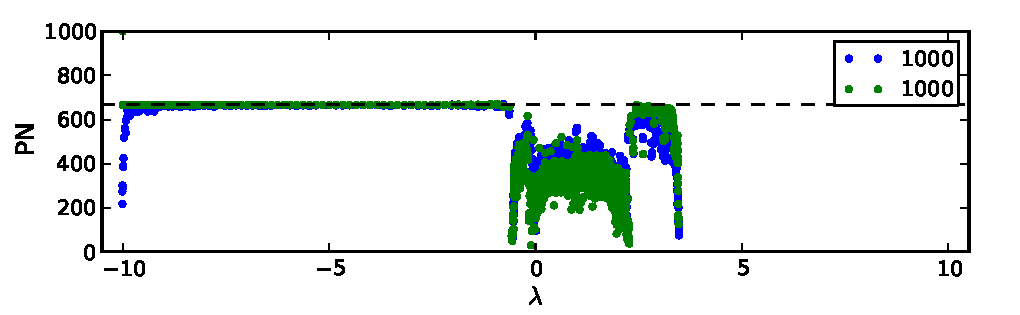
\includegraphics{pta_anderson_b5_ROD_VS_SC}
    \caption{$PN$ vs eigenvalue $\lambda$, for $b=5$, $s=0.1$ ,$N=1000$. 
    The green points are for the conserving model, the blue for the non-conserving.
    The main (and very important!) difference between the two, is on the lowermost $\lambda$, in which
    $PN$ does not go to zero although the $DOS$ does go to zero. There is also
    a solitary green point on $N=1000$, which is the ergodic state.}
    \label{fig:ROD}
\end{figure}


%%%%%%%%%%%%%%%%%%%%%%%%%%%%%%%%%%%%%%%%%%%%%%%%%%%%%%%%%%%%%%%%%%%%
\sect{strong disorder}


We now put moderately stronger disorder. We see two effects. On the one hand, the $PN$'s seem closer
to our theoretical $\ell$ prediction. On the other hand, we can visually see
broadening of the band on both sides. For very strong disorder the band structure disappears all together.





%%%%%%%%----------%%%%%%%%
%%%%%%%%  figure  %%%%%%%%
%%%%%%%%----------%%%%%%%%
\begin{figure}[H]
    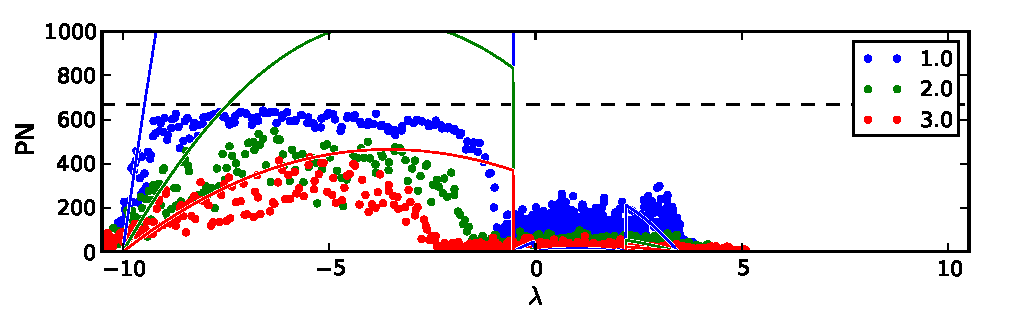
\includegraphics{pta_anderson_strong}\\
    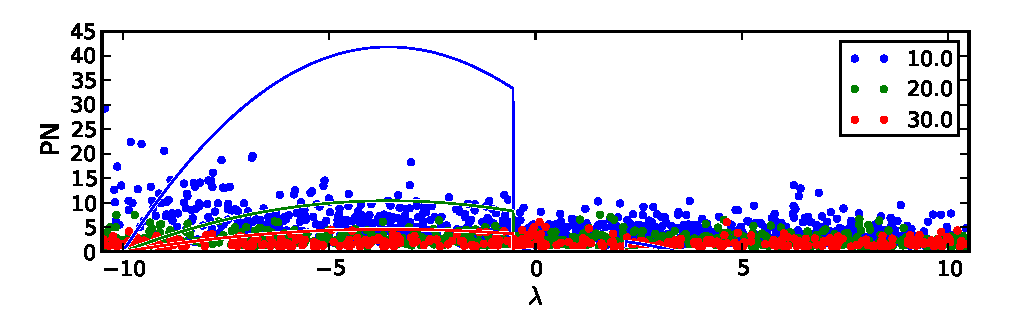
\includegraphics{pta_anderson_very_strong}\\
    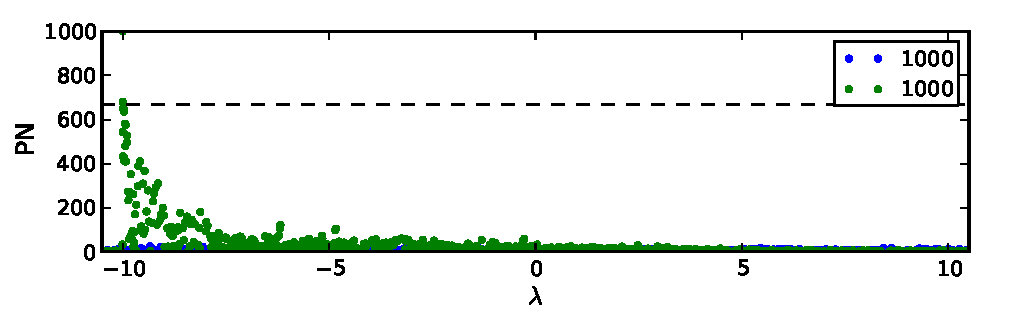
\includegraphics{pta_anderson_b5_s10_ROD_VS_SC}
    \caption{Top two plots: $PN$ vs eigenvalue $\lambda$, for $b=5$, $s={1,2,3,10,20,30}$ ,$N=1000$. 
    For the medium strength ($s={1,2,3}$), we see better fitting to our prediction (since $\ell \approx N$),
    but we also see widening of the bands. In the very strong disorder, the band features are lost.
    In the third plot, $s=10$, and we have off-diagonal disorder, once conserving (green) and once not.
    Luckily, we do not lose the "extended"- diffusive modes in the conserving disorder.}
    \label{fig:strong}
\end{figure}





\bibliographystyle{apsrev4-1}
\bibliography{../bibliography/jarondl,../bibliography/custom-longbib}


\end{document}
